\section{Plano de Marketing}

\subsection{Descrição dos produtos e serviços}

\subsubsection*{Controlador de Voo}

O controlador de voo consiste num dispositivo de aproximadamente 
$7$ x $3$ x $1.5$ $cm^3$, o qual inclui diversas entradas e saídas, 
como no diagrama a seguir:

\begin{figure}[H]
\centering
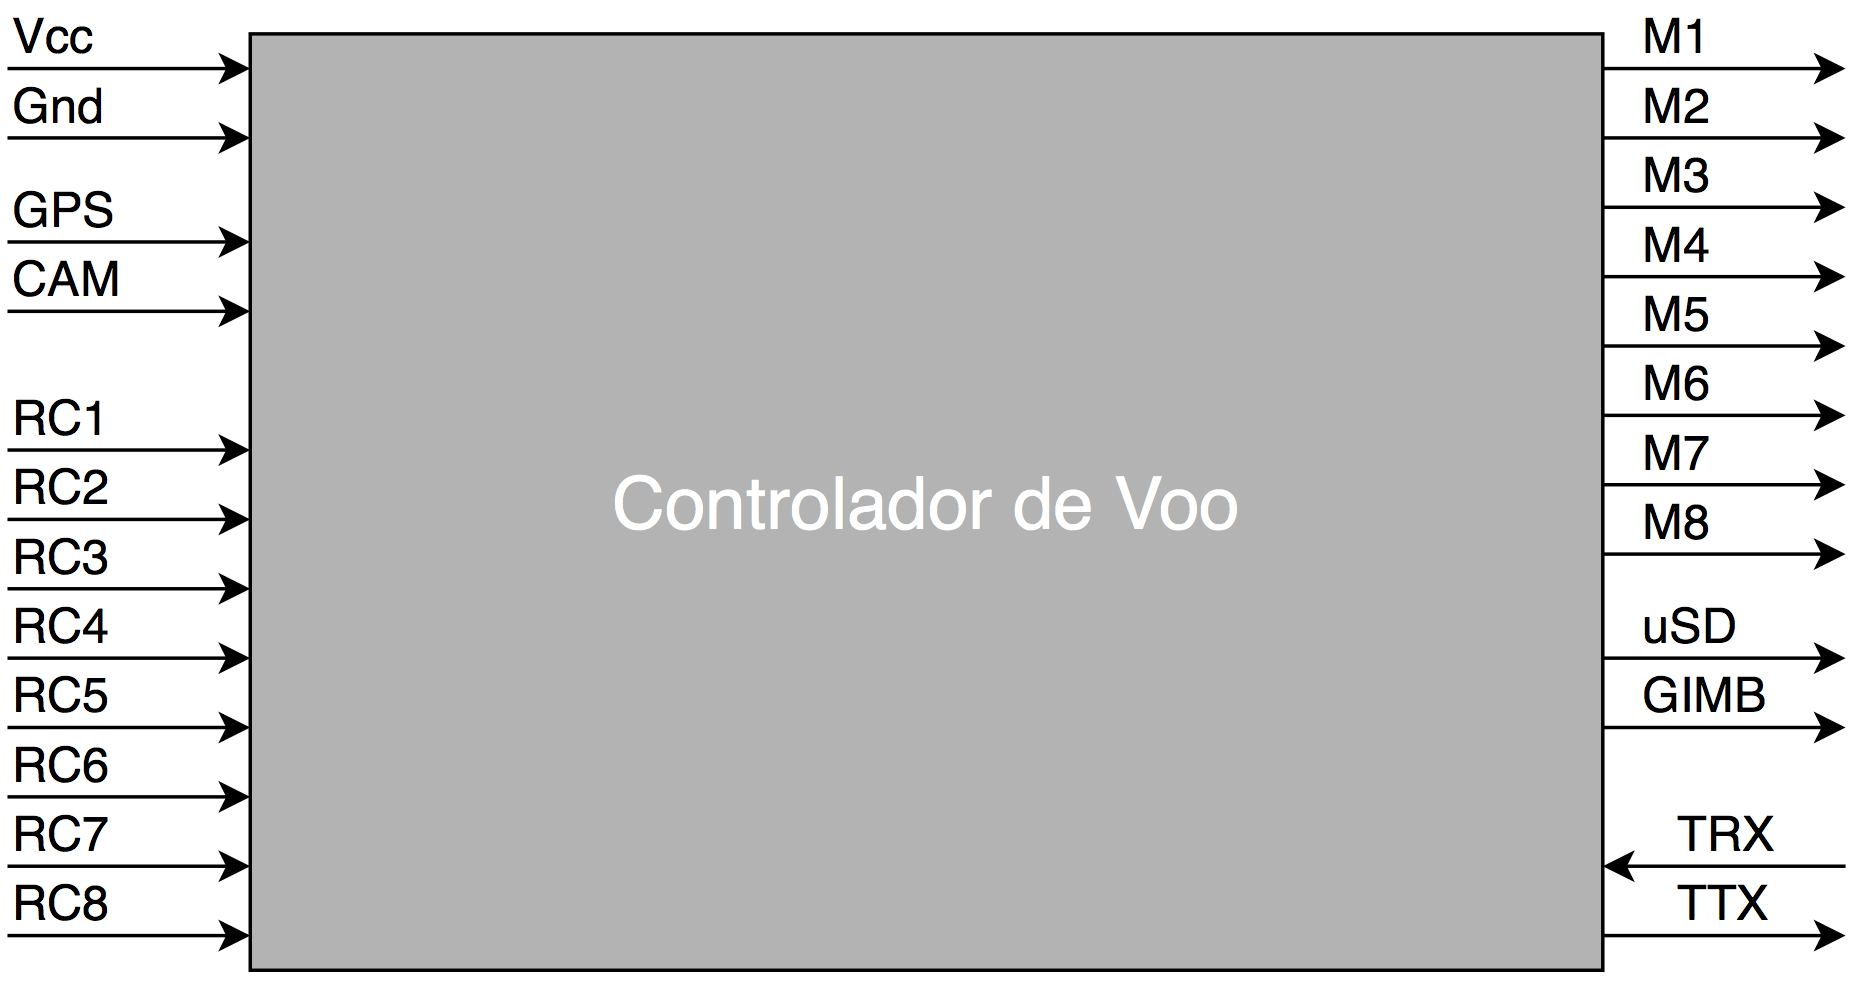
\includegraphics[width=\textwidth]{fcdiagrama.png}
\caption{Diagrama de entradas e saídas do controlador de voo.}
\label{fig:fcdiagrama}
\end{figure}

Descrição das entradas e saídas:
\begin{itemize}
	\item Vcc: Alimentação +12 Volts
	\item Gnd: Alimentação terra
	\item GPS: Entrada de dados de módulo de GPS
	\item CAM: Entrada de dados de módulo de câmera
	\item RC1..RC8: Entrada de dados de cada um dos 8 possíveis 
	canais de rádio controle
	\item M1..M8: Saídas de comandos para cada um dos possíveis 8 motores
	\item uSD: Saída de dados para cartão SD (caixa preta)
	\item GIMB: Saída de comandos para \emph{Gimbal} (sistema de estabilização de câmera)
	\item TRX: Entrada de dados de \emph{link} digital de telemetria
	\item TTX: Saída de dados de \emph{link} digital de telemetria
\end{itemize}

Internamente, o controlador possui um microcontrolador que é 
responsável pela execução do \emph{firmware} de controle, giroscópio 
3D (ou seja, nos eixos $x, y$ e $z$), acelerômetro 3D, magnetômetro 
3D, barômetro e termômetro. O mínimo necessário para voar é um rádio
controle de 4 canais, uma bateria de polímero de lítio para 
alimentação do \emph{Drone} inteiro e ao menos 4 motores.

Caso o usuário deseje, pode-se conectar um módulo de GPS externo, 
permitindo navegação autônoma baseada em coordenadas; um cartão
SD para permitir gravação de dados e fotos/vídeos; um \emph{link}
digital para comunicação com \emph{smartphone} ou computador em 
tempo real; uma câmera; um \emph{Gimbal}, que permite estabilização 
da câmera (compensação dos movimentos do \emph{Drone}); motores 
adicionais (até 8) e canais de rádio adicionais (até 8).

\subsubsection*{Prestação de Serviços}

No ramo da prestação de serviços de consultoria e projetos em \emph{Drones},
algumas das atividades que podem ser executadas são:

\subsubsection*{Ramo Florestal}

\begin{itemize}
	\item Vistoria de propriedades para compra e venda
	\begin{itemize}
		\item Análise da qualidade de plantio
		\item Alinhamento do plantio
		\item Mapeamento topográfico
	\end{itemize}
	\item Monitoramento de pragas
	\begin{itemize}
		\item Identificação de falhas de aplicação de defensivos agrícolas
		\item Identificação de áreas com pragas
	\end{itemize}
	\item Mapeamento de falhas
	\item Avaliação de incêndios
\end{itemize}

\subsubsection*{Agricultura}

\begin{itemize}
	\item Análise de plantio
	\item Controle e identificação de pragas
	\begin{itemize}
		\item Identificação de falhas de aplicação de defensivos agrícolas
		\item Identificação de áreas com pragas ou deficiências nutricionais
	\end{itemize}
	\item Inspeção de lavouras
	\item Laudos agronômicos de interesse econômico
	\item Mapeamento de resíduos
	\item Avaliação de experimentos agrícolas
	\item Cálculo do índice vegetativo da plantação
\end{itemize}

\subsubsection*{Ambiental}

\begin{itemize}
	\item Monitoramentos de recuperação ambiental
	\item Laudos de conformidade de APP
	\item Avaliação ambiental e de dano ambiental
	\item Monitoramento de desmatamento
\end{itemize}

\subsubsection*{Construção Civil}

\begin{itemize}
	\item Inspeções em áreas de alto risco
	\begin{itemize}
		\item Laudos de acidentes
		\item Mapeamento de áreas afetadas e de risco
		\item Registro de danos
	\end{itemize}	
	\item Lançamento de novos empreendimentos
	\begin{itemize}
		\item Fotos de simulação da sacada para cada andar do prédio
		\item Fotos para publicidade
	\end{itemize}	
	\item Mapeamento urbanístico
	\item Acompanhamento e inspeção de obras
	\begin{itemize}
		\item Controle de qualidade
		\item Atualizações semanais
		\item Comprovação de trabalho realizado		
	\end{itemize}
	\item Topografia
\end{itemize}

\subsubsection*{Cinematografia}

\begin{itemize}
	\item Fotos de empresas e lojas
	\item Fotos de locais de eventos
	\item Publicidade aérea
	\item Anúncios comerciais
	\item Filmagem de comerciais
	\item Fotos de eventos
	\item Filmagem por ângulos não convencionais
	\item Possibilidade de acompanhamento de esportes (F1, atletismo, futebol etc)
\end{itemize}

\subsection{Preço}

% Avaliar o preço a ser cobrado por cada produto ou serviço e comparar com o que é 
% praticado atualmente no mercado.

O preço do produto deve ser barato o suficiente para vencer os 
atuais concorrentes internacionais que vendem seus produtos no 
Brasil através de revendedores. De acordo com as pesquisas, o 
preço do controlador em si deve custar em torno de R\$800 para 
ganhar mercado de maneira rápida por ser mais barato. Entretanto, 
se analisarmos os canais oficiais de venda, o preço do produto 
pode ser estipulado em torno de R\$1100, o que ainda garante o 
fator melhor preço. Sendo assim, uma estratégia de entrada do 
produto no mercado pode ser dada por um preço em torno de R\$1000 com o 
diferencial dos serviços agregados, como garantia em todo território 
nacional, rapidez de entrega e suporte nacional, tanto para produto 
como consultoria básica de utilização, de modo a conquistar uma 
rede de clientes e promover o nome da empresa no nicho desejado.

Para os serviços nas áreas florestais, agricultura, ambiental, mineração, 
industrial, construção civil, empreendimentos imobiliários, 
obras e cinegrafia o preço é atrelado ao tamanho do projeto e 
à quantidade necessária de homem $\times$ hora de trabalho, que é o principal 
gasto neste ramo. Ademais, este tipo de serviço deve avaliar o preço
e o tempo que seria gasto para ser executado por meios normais,
baseando o preço final também neste parâmetro.
No ramo da cinegrafia, um dos mercados considerados 
mais promissores, uma filmagem de casamento custa em média 
R\$ 4000 dependendo da qualidade do equipamento e tempo de filmagem.

\subsection{Estratégias promocionais}

% Ações que tem como objetivo apresentar, informar, convencer ou lembrar os clientes
% de comprar os produtos: propaganda física/online, amostra grátis, catálogos, descontos,
% adSense, participação em feiras e eventos (!!! agricultura).

É importante destacar aqui a estratégia de entrada no mercado. 
A empresa deve adquirir um cliente com nome conhecido, sem fins 
lucrativos, por um preço reduzido, para prestar o primeiro serviço e 
se adequar ao mercado em si. Após este primeiro projeto piloto, a 
empresa possui um caso de sucesso (um "\emph{case}") para utilizar como 
base nas propagandas e divulgações de produto, além de experiência 
prévia que diminuirá as chances de problemas nos projetos seguintes.

Também são necessários canais \emph{online} (website, redes sociais, 
anúncios em sites relacionados etc.) para divulgação de vídeos 
promocionais e descrição de serviços e produtos ofertados, além de 
eventuais promoções. Como parte do potencial público encontra-se no 
interior ou em regiões afastadas da localização do negócio devido à baixa 
competitividade, é de suma importância um bom canal de atendimento a 
distância, com respostas rápidas e de qualidade. 

As feiras e eventos de \emph{Drones} espalhadas pelo Brasil são fatores chave para 
divulgação da empresa e troca de conhecimento. Feiras agrícolas não devem 
ser esquecidas, pois são um mercado potencialmente grande que movimenta 
muito capital anualmente e podem proporcionar um faturamento elevado para a empresa. 

\subsection{Estrutura de comercialização}

% Canais de distribuição. Vendedores, distribuidores etc. Pensar no comportamento dos
% clientes.

O primeiro canal de vendas seria o \emph{e-commerce}, pois atinge uma maior 
quantia de pessoas com um menor custo, além de permitir táticas agressivas 
de publicidade e frete para todo o país. Além disto, é importante ter um 
escritório localizado em uma grande cidade chave, como será abordado 
posteriormente. É importante também montar uma rede de revendedores e 
distribuidores de \emph{hardware} pelo país, em cidades que permitam 
garantir uma rapidez no suporte e entrega de produtos, visando expandir o 
nome da marca nos nichos desejados, como dos \emph{hobbystas} por exemplo. 
Vale ressaltar também a importância de stands em eventos de \emph{Drones}, visando 
a divulgação da marca, mostra de produtos, mostra de serviços prestados e 
compartilhamento de conhecimento, o que agrega muito à imagem da empresa.
Em um primeiro momento, também é necessário que consultores busquem em campo 
novos clientes, indo em regiões de mercado alvo forte para propor projetos e 
mostrar serviços e produtos que eles não conheciam, mas que podem ser 
suficientemente interessantes para serem adquiridos.

\subsection{Localização do Negócio}

% Escolher e justificar uma localização. Cidade grande, provavelmente? Como fornecer
% serviços a agricultores? Realmente precisa de um lugar fixo no começo?

Como dito anteriormente, é importante estabelecer um escritório em uma cidade 
grande chave, como o próprio Rio de Janeiro, de modo a permitir o recebimento de 
produtos internacionais necessários ao desenvolvimento do controlador de voo, 
além de mão de obra qualificada para projetos, pesquisa e desenvolvimento. 
Ademais, as grandes capitais possuem a melhor rede de infraestrutura para se 
montar este tipo de negócio, além dos serviços aéreos para a maior parte do 
pais, o que é de suma importância para expandir o mercado atacado e de serviços.
